\section{Design}
%
%%%%%%%%%%%%%%%%%%%%%%%%%%%%%%%%%%%%%%%%%%%%%%%%%%%%%%%%%%%
\subsection{Judgments and transcriptions}
%
%%%%%%%%%%%%%%%%%%%%%%%%%%%%%%%%%%%%
\subsubsection{Judgement assumptions}
%
On the one hand, HJ methods have their assumptions rooted in the Classical Test Theory (CTT), where an individual's observed score is composed of a "true score", and a random measurement error. Moreover, the true score is defined as the expected value of the score under an infinite number of independent test administrations\footnote{\url{https://www.ncme.org/resources/glossary}}.

On the other hand, CJ methods hinges on two principles: the law of comparative judgments \citep{Thurstone_1927}, and the consensus of judges \citep{Lesterhuis_2018}. Under the former, the outcome of a comparison, i.e. a relation of preference, is determined by the perceived difference between the discriminal processes of pairs. A \textit{discriminal process}, is the assumed physiological impact that a stimulus has on a listener. However, since this impact cannot be measured directly, we are forced to make some assumption about such process. The minimal assumption we can make is that the process' ordering on the psychological continuum, is the same as the stimulus' ordering that cause them. Moreover, as frequently observed in the field of psycho-physics, since the relationship between stimulus and its impact is not one-to-one, we are also forced to assume the impact has a dispersion/variability, called the \textit{discriminal dispersion}\footnote{for a detailed explanation of the law, see \citet{Thurstone_1927, Verhavert_2018} (p. 22-29)}. Finally, the latter principle indicates the shared consensus across judges adds to the validity of the method \citep{Lesterhuis_2018}. This claim is supported by the fact that different listeners differ in the focus and broadness of their judgments \citep{Lesterhuis_2018}, and that each representation is assessed by multiple judges, implying the final score is a reflection of the judges’ collective expertise \citep{Pollitt_2012b}. This only means that by combining various judgments, we come closer to the "true" rankings of SI \citep{Lee_et_al_2014}.
%
%
%%%%%%%%%%%%%%%%%%%%%%%%%%%%%%%%%%%%
\subsubsection{Procedures} \label{ss_sect:proc}
%
The HJ procedure consisted on two psycho-linguistic\footnote{the science	of human language production, comprehension, and acquisition \citep{Levelt_1993}.} stages: (1) select and mentally represent the stimulus' information, independent of other stimuli, and (2) rate the representation, according to a task. Therefore, under this procedure, listeners rate the stimulus' SI in an absolute manner, with an 100-point scale going from "very unintelligible" ($0$) to "very intelligible" ($100$) \citep{Boonen_et_al_2021, Faes_et_al_2021}.

In contrast, CJ is composed of three interrelated psycho-linguistic stages: (1) select and mentally represent the information of the pairs, (2) compare and weigh their relevant information, and (3) rate which representation is preferred, according to a task \citep{vanDaal_2020}. As a result, in CJ-D, the listeners rate a pair of stimuli in a dichotomous way, i.e. if stimulus A is more intelligible than B you observe a one in the outcome variable, and zero otherwise \citep{Bradley_et_al_1952}. On the other hand, under CJ-O, the listeners rate both stimuli on a 5-point ordinal scale\footnote{evidence on the quality, reliability, and validity benefits of a 5-point scale can be found in \citet{Revilla_et_al_2014}.} where the outcome variable maps to the following preference relationships: $A>>B$, $A>B$, $A=B$, $A<B$, $A<<B$, where $>>$, $>$, $<<$, $<$, and $=$ symbols indicate the level of preference and indifference between the pairs, respectively \citep{Tutz_1986, Agresti_1992}.
%
%
%%%%%%%%%%%%%%%%%%%%%%%%%%%%%%%%%%%%
\subsubsection{Experimental settings} \label{ss_sect:expset}
%
On both procedures, the experimental settings for the \textbf{judgment task} followed the next steps \citep{Boonen_et_al_2020, Boonen_et_al_2021}:
%
\begin{enumerate}
	\item the listener took a seat in front of a computer screen, located at his(her) home, workplace, or the experimental laboratory, and open Comproved\footnote{\url{https://comproved.com/en/a}, a software tool developed by the University of Antwerp designed to perform comparative judgments.}
	%
	\item two set of instructions were presented on the computer screen:
	\begin{enumerate}
		\item how to perform the task, and
		\item the aspects not to consider for the task.
	\end{enumerate}
	%
	\item the listener hear the stimuli through high quality headphones, set at a comfortable volume.
	%
	\item the listener rate which stimulus sounded better by selecting the appropriate button, for CJ-D and CJ-O tasks, or select a score from a slider on the computer screen, for the HJ task.
\end{enumerate}
%
\begin{figure}[h]
	\centering
	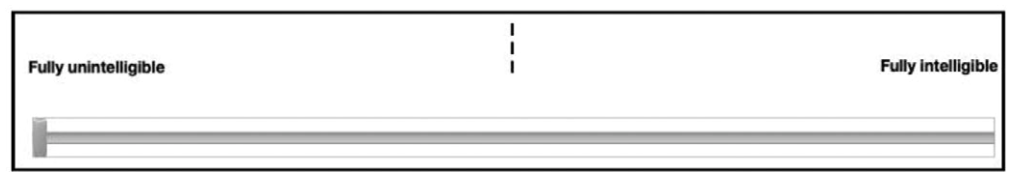
\includegraphics[width=0.8\linewidth]{slider.png}
	%
	\caption[Slider for the HJ task.]%
	{Slider for the HJ task. Extracted from \citet{Boonen_et_al_2021}.}
	\label{fig:slider}
\end{figure}
%
Observational evidence indicate the HJ procedure might suffer from anchoring effects\footnote{a bias in decision that occurs when people anchor their decisions around a reference point, and adjust their choices relative to it \cite{Baddeley_2017, Kahneman_2013}.}, or issues with the default option of the slider. About the former, the anchoring seem to happen when listeners consider the previous assessment as a reference point for the next, effectively turning the task into a comparative rating, similar to CJ. About the latter, as the default setting for the slider is located on the far left for each new assessment (as seen in Figure \ref{fig:slider}), it is likely that such setting might impact the rating procedure\footnote{compelling evidence on how default settings impact several decision process can be found in \citet{Kahneman_2013} and \citet{Johnson_et_al_2003}.}. Considering the previous, care is taken to randomize the display of stimuli within each listener, in order to minimize both issues. However, the researcher recognizes that a better approach to face the latter would be to randomize the default setting of the slider, but this will not be investigated on the current research. 

Finally, for the \textbf{transcription task}, the followed steps were similar to the previous. However, at the fourth step, the listeners did not rated the stimulus, but rather produced their orthographic transcriptions.
%
%
%%%%%%%%%%%%%%%%%%%%%%%%%%%%%%%%%%%%%%%%%%%%%%%%%%%%%%%%%%%
\subsection{Stimuli}
%
The stimuli consisted of children's utterances (sentences of similar length) recovered from a larger corpus of \textit{spontaneously spoken speech} collected by CLiPS over the last twenty years. More specifically, we use a portion of the corpus that consisted of $10$ utterances recordings for $32$ 7-year old children, telling a story cued by the picture book "Frog, where are you" \citep{Mayer_1969} to a caregiver "who does not know the story". The utterances were selected making sure they did not have syntactically ill-formed or incomplete sentences, any background noise, cross-talk, long hesitations, revisions or non-words \citep{Boonen_et_al_2021}. As a result, the data set consisted in a total of $320$ utterances\footnote{under the Design of Experiments (DoE) literature, we would say we have $32$ experimental units with $10$ replicate runs each, making a total of $320$ experimental runs. As it is defined in \citet{Lawson_2015}, an experimental unit is the item under study upon which something is changed, and a replicate run is the experiment conducted with the same factor settings, but using different experimental units.}, that were presented to the listeners in a random order based on a pairing algorithm implemented in Comproved.

Similar designs were used by \citet{Boonen_et_al_2020} and \citet{Faes_et_al_2021}. However, in the former case the number of samples were low, while in the latter, the design was unbalanced and not conducive to appropriate inferences from a pairwise comparison.
%
%
%%%%%%%%%%%%%%%%%%%%%%%%%%%%%%%%%%%%%%%%%%%%%%%%%%%%%%%%%%%
\subsection{Comparisons / assessments}
%
In terms the number of comparison per representation (stimulus) required, \citet{Verhavert_2018} provided compelling evidence that under CJ, between $17$ and $20$ comparisons were enough to achieved a Scale Separation Reliability (SSR) of $0.80$. The current research uses the higher end of such values ($20$). On the other hand, based on \textcolor{red}{[source]} only $5$ assessments per representation were required under the HJ method, \textcolor{red}{to achieve what?}. Therefore, we use the same number of assessments under HJ\footnote{Under DoE literature, this implies we will have $20$ and $5$ duplicates for each replicate run, under the CJ and HJ procedures, respectively. As defined in \citet{Lawson_2015}, duplicates are repeated measurements of the same experimental unit from one run, where it is possible the measured dependent variable vary among duplicates due to measurement error.}.
%
%
%%%%%%%%%%%%%%%%%%%%%%%%%%%%%%%%%%%%%%%%%%%%%%%%%%%%%%%%%%%
\subsection{Judges and transcribers} \label{s_sect:JandT}
%
The generation of the ratings required the participation of $180$ judges (listeners). The judges were students from the Toegepaste Taalkunde bachelor or from the Taal- en Letterkunde master's degree. On both cases, the judges participated in the procedure as part of their course credit. \textcolor{blue}{We expect the CJ tasks to be 4-times more demanding, in terms of time and effort, than the HJ task, therefore, we allocate 4-times more judges in such task}. Table \ref{tab:allocation} describes the judge allocation, the total number of judgments, and the number of judgments per judge.
%
\begin{table}[h!]
	\centering
	\begin{tabular}{|| c c | c | c c| c | c | c || } 
		\hline
		& & Number & \multicolumn{2}{c |}{Number (per stimuli)} & Total & Number & Judgments \\ [0.5ex]
		\cline{4-5}
		& Method & Utterances &  assessments & comparisons & judgments & judges & per judge \\ [0.5ex] 
		\hline\hline
		1 & CJ-D & 320 & n.a. & 20 & 6400 & 80 & 80 \\ 
		2 & CJ-O & 320 & n.a. & 20 & 6400 & 80 & 80 \\
		3 & HJ & 320 & 5 & n.a. & 1600 & 20 & 80 \\
		\hline
		\multicolumn{4}{l}{\footnotesize{n.a.= not applicable}}
	\end{tabular}
	\caption{Design to rate $320$ stimuli per judgment method.}
	\label{tab:allocation}
\end{table}

On the other hand, for the transcription task, $100$ transcribers participated in the experiment. The participants and stimuli were divided into five groups. As a consequence, each group of $20$ students ($100/5$) transcribed $64$ stimuli on their series ($320/5$), resulting in $20$ transcriptions per utterance ($64 \times 100 / 320$)\footnoteref{foot:doe}}.
%
%